\newpage
\section{Versuchsdurchführung}
\label{sec:durchfuerung}
%Ausführliche Beschreibung der eigenen Versuchsdurchführung in Sätzen.
%- Einbindung der eigenen Beobachtungen und der Notizen aus dem
%Beobachtungsprotokoll.
%- Benennung der ggf. während des Versuches aufgetretenen Schwierigkeiten,
%Probleme oder unerwarteten Phänomene.
Zu Beginn des Versuches wird die Zirkulationsapparatur, zu sehen unter Abb. \ref{fig:aufbau}, mit \SI{65}{\milli \liter} reinem Ethanol befüllt. Infolgedessen wird die Apparatur mittels Innenheizung, eingestellt auf \SI{70}{\celsius}, in Betrieb genommen. Die mittels Trafo geregelte Spannung der Heizung darf dabei den Grenzwert von \SI{180}{\volt} nicht überschreiten. Die Flüssigkeit in der Zirkulationsapparatur beginnt zu sieden und der entstehende Dampf wird mittels Kühler in einem separaten Abschnitt der Apparatur in ein Siphon geleitet. Um festzustellen ob sich das Stoffsystem in der Apparatur im thermodynamischen Gleichgewicht befindet, wird die Temperatur beobachtet. Verhält sich die Temperatur nahezu konstant ist, ist von einem Gleichgewicht auszugehen und es kann die Zusammensetzung der Flüssig- und der Gasphase untersucht werden. Hierfür wird die Heizung temporär ausgeschaltet und jeweils ein Teil der Flüssigphase und Teil des Dampfkondensats mit separaten Spritzen entnommen. Die neue zu untersuchende Zusammensetzung mit den entsprechenden Volumina, die dem System zuzugeben sind, sind am Versuchsaufbau schriftlich festgehalten. Es ist darauf zu achten, dass die gleichen Volumina der nicht vorgelegten Komponente zugegeben werden, wie dem System entnommen wurden.

Um den azeotropen Punkt des Ethanol-Cyclohexan-Gemisches zu vermeiden, wird sich im Praktikum von beiden Seiten des azeotropen Punktes mit der Zusammensetzung angenähert. Ist von einer Seite der azeotrope Punkt nahezu erreicht, wird der Aufbau entleert, mit Luft trocken geblasen und mit zuvor nicht vorgelegten Komponente befüllt. Die Menge an Ethanol, die zugeführt werden muss, ist ebenfalls am Versuchsstand schriftlich notiert.

\begin{figure}[h!]
	\centering
	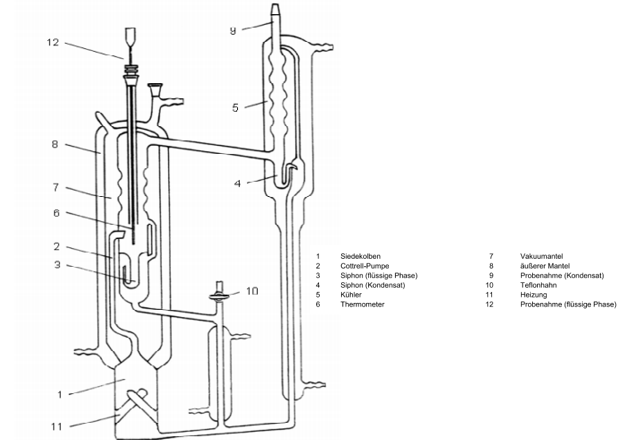
\includegraphics[width=0.9\textwidth]{img/aufbau}
	\caption{Skizze der Zirkulationsapparatur }
	\label{fig:aufbau}
\end{figure}
\FloatBarrier
%Ende